\documentclass[]{article}
\usepackage{amsfonts, amssymb, amsmath}
\usepackage{graphicx}
\begin{document}
\providecommand{\pr}[1]{\ensuremath{\Pr\left(#1\right)}}
\providecommand{\prt}[2]{\ensuremath{p_{#1}^{\left(#2\right)} }}        % own macro for this question
\providecommand{\qfunc}[1]{\ensuremath{Q\left(#1\right)}}
\providecommand{\sbrak}[1]{\ensuremath{{}\left[#1\right]}}
\providecommand{\lsbrak}[1]{\ensuremath{{}\left[#1\right.}}
\providecommand{\rsbrak}[1]{\ensuremath{{}\left.#1\right]}}
\providecommand{\brak}[1]{\ensuremath{\left(#1\right)}}
\providecommand{\lbrak}[1]{\ensuremath{\left(#1\right.}}
\providecommand{\rbrak}[1]{\ensuremath{\left.#1\right)}}
\providecommand{\cbrak}[1]{\ensuremath{\left\{#1\right\}}}
\providecommand{\lcbrak}[1]{\ensuremath{\left\{#1\right.}}
\providecommand{\rcbrak}[1]{\ensuremath{\left.#1\right\}}}
\newcommand{\sgn}{\mathop{\mathrm{sgn}}}
\providecommand{\abs}[1]{\left\vert#1\right\vert}
\providecommand{\res}[1]{\Res\displaylimits_{#1}} 
\providecommand{\norm}[1]{\left\lVert#1\right\rVert}
%\providecommand{\norm}[1]{\lVert#1\rVert}
\providecommand{\mtx}[1]{\mathbf{#1}}
\providecommand{\mean}[1]{E\left[ #1 \right]}
\providecommand{\cond}[2]{#1\middle|#2}
\providecommand{\fourier}{\overset{\mathcal{F}}{ \rightleftharpoons}}
\newenvironment{amatrix}[1]{%
  \left(\begin{array}{@{}*{#1}{c}|c@{}}
}{%
  \end{array}\right)
}
%\providecommand{\hilbert}{\overset{\mathcal{H}}{ \rightleftharpoons}}
%\providecommand{\system}{\overset{\mathcal{H}}{ \longleftrightarrow}}
	%\newcommand{\solution}[2]{\textbf{Solution:}{#1}}
\newcommand{\solution}{\noindent \textbf{Solution: }}
\newcommand{\cosec}{\,\text{cosec}\,}
\providecommand{\dec}[2]{\ensuremath{\overset{#1}{\underset{#2}{\gtrless}}}}
\newcommand{\myvec}[1]{\ensuremath{\begin{pmatrix}#1\end{pmatrix}}}
\newcommand{\mydet}[1]{\ensuremath{\begin{vmatrix}#1\end{vmatrix}}}
\newcommand{\myaugvec}[2]{\ensuremath{\begin{amatrix}{#1}#2\end{amatrix}}}
\providecommand{\rank}{\text{rank}}
\providecommand{\pr}[1]{\ensuremath{\Pr\left(#1\right)}}
\providecommand{\qfunc}[1]{\ensuremath{Q\left(#1\right)}}
	\newcommand*{\permcomb}[4][0mu]{{{}^{#3}\mkern#1#2_{#4}}}
\newcommand*{\perm}[1][-3mu]{\permcomb[#1]{P}}
\newcommand*{\comb}[1][-1mu]{\permcomb[#1]{C}}
\providecommand{\qfunc}[1]{\ensuremath{Q\left(#1\right)}}
\providecommand{\gauss}[2]{\mathcal{N}\ensuremath{\left(#1,#2\right)}}
\providecommand{\diff}[2]{\ensuremath{\frac{d{#1}}{d{#2}}}}
\providecommand{\myceil}[1]{\left \lceil #1 \right \rceil }
\newcommand\figref{Fig.~\ref}
\newcommand\tabref{Table~\ref}
\newcommand{\sinc}{\,\text{sinc}\,}
\newcommand{\rect}{\,\text{rect}\,}
%%
%	%\newcommand{\solution}[2]{\textbf{Solution:}{#1}}
%\newcommand{\solution}{\noindent \textbf{Solution: }}
%\newcommand{\cosec}{\,\text{cosec}\,}
%\numberwithin{equation}{section}
%\numberwithin{equation}{subsection}
%\numberwithin{problem}{section}
%\numberwithin{definition}{section}
%\makeatletter
%\@addtoreset{figure}{problem}
%\makeatother

%\let\StandardTheFigure\thefigure
\let\vec\mathbf

1.4.1. The equation of the perpendicular bisector of $BC$ is
\begin{align}
{\myvec{\vec{B}-\vec{C}}}^\top \myvec{\vec{x} - \frac{\vec{B}+\vec{C}}{2}} = 0
\end{align}
Substitute numerical values and find the equations of the perpendicular bisectors of $AB$, $BC$ and $CA$.

\solution
It is given that
\begin{align}
\vec{A} = \myvec{1\\-1}, \vec{B}=\myvec{-4\\6}, \vec{C}=\myvec{-3\\-5}
\end{align}
\begin{enumerate} 
\item {The equation of perpendicular bisector of $BC$ is given as
\begin{align}
{\myvec{\vec{B}-\vec{C}}}^\top \myvec{\vec{x} - \frac{\vec{B}+\vec{C}}{2}} &= 0 \\
{\myvec{\myvec{-4\\6}-\myvec{-3\\-5}}}^\top \myvec{\vec{x} - \frac{1}{2} \myvec{\myvec{-4\\6}+\myvec{-3\\-5}}  } &= 0 \\
{\myvec{-1\\11}}^\top \myvec{\vec{x} - \frac{1}{2}\myvec{-7\\1}} &= 0\\
\myvec{-1&11} \myvec{\vec{x} - \frac{1}{2}\myvec{-7\\1}} &= 0\\
\myvec{-1&11}\vec{x} &= \frac{1}{2}\myvec{-1&11}\myvec{-7\\1}\\
\myvec{-1&11}\vec{x} &= \frac{7+11}{2}\\
\myvec{-1&11}\vec{x} &= 9
\end{align}}
\item {Similarly, the equation of the perpendicular bisector of $AB$ is given as
\begin{align}
{\myvec{\vec{B}-\vec{A}}}^\top \myvec{\vec{x} - \frac{\vec{B}+\vec{A}}{2}} &= 0 \\
{\myvec{\myvec{-4\\6}-\myvec{1\\-1}}}^\top \myvec{\vec{x} - \frac{1}{2}\myvec{\myvec{-4\\6}+\myvec{1\\-1}}  } &= 0 \\
{\myvec{-5\\7}}^\top \myvec{\vec{x} - \frac{1}{2}\myvec{-3\\5}} &= 0\\
\myvec{-5&7} \myvec{\vec{x} - \frac{1}{2}\myvec{-3\\5}} &= 0\\
\myvec{-5&7}\vec{x} &= \frac{1}{2}\myvec{-5&7}\myvec{-3\\5}\\
\myvec{-5&7}\vec{x} &= \frac{15+35}{2}\\
\myvec{-5&7}\vec{x} &= 25
\end{align}}
\item {Similarly, the equation of the perpendicular bisector of $AC$ is given as
\begin{align}
{\myvec{\vec{A}-\vec{C}}}^\top \myvec{\vec{x} - \frac{\vec{A}+\vec{C}}{2}} &= 0 \\
{\myvec{\myvec{1\\-1}-\myvec{-3\\-5}}}^\top \myvec{\vec{x} - \frac{1}{2} \myvec{\myvec{1\\-1}+\myvec{-3\\-5}}  } &= 0 \\
{\myvec{4\\4}}^\top \myvec{\vec{x} - \frac{1}{2}\myvec{-2\\-6}} &= 0\\
\myvec{4&4}\myvec{\vec{x}+\myvec{1\\3}} &= 0\\
\myvec{4&4}\vec{x} &= -\myvec{4&4}\myvec{1\\3}\\
\myvec{4&4}\vec{x} &= -4-12 \\
\myvec{4&4}\vec{x} &= -16 \\
4\myvec{1&1}\vec{x} &= -16 \\
\myvec{1&1}\vec{x} &= -4
\end{align}}
\end{enumerate}
\begin{figure}
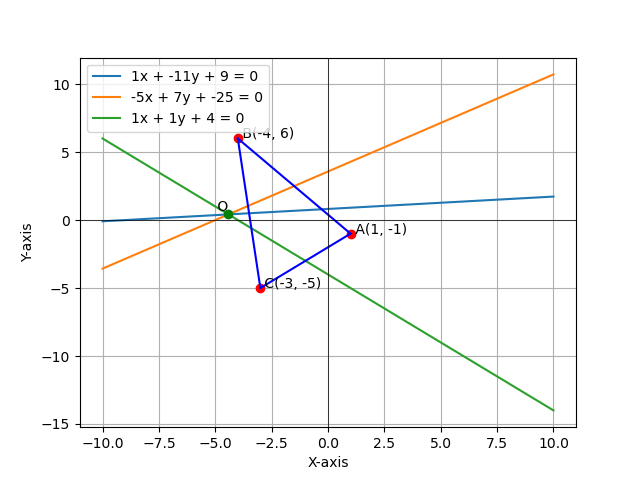
\includegraphics{figs/perp_bisector.png}
\caption{Perpendicular bisectors of AB, BC and CA}
\end{figure}
\end{document}
